\documentclass{beamer}

% xcolor and define colors -------------------------
\usepackage{xcolor}

% https://www.viget.com/articles/color-contrast/
\definecolor{purple}{HTML}{5601A4}
\definecolor{navy}{HTML}{0D3D56}
\definecolor{ruby}{HTML}{9a2515}
\definecolor{alice}{HTML}{107895}
\definecolor{daisy}{HTML}{EBC944}
\definecolor{coral}{HTML}{F26D21}
\definecolor{kelly}{HTML}{829356}
\definecolor{cranberry}{HTML}{E64173}
\definecolor{jet}{HTML}{131516}
\definecolor{asher}{HTML}{555F61}
\definecolor{slate}{HTML}{314F4F}

% Mixtape Sessions
\definecolor{picton-blue}{HTML}{00b7ff}
\definecolor{violet-red}{HTML}{ff3881}
\definecolor{sun}{HTML}{ffaf18}
\definecolor{electric-violet}{HTML}{871EFF}

% Main theme colors
\definecolor{accent}{HTML}{00b7ff}
\definecolor{accent2}{HTML}{871EFF}
\definecolor{gray100}{HTML}{f3f4f6}
\definecolor{gray800}{HTML}{1F292D}


% Beamer Options -------------------------------------

% Background
\setbeamercolor{background canvas}{bg = white}

% Change text margins
\setbeamersize{text margin left = 15pt, text margin right = 15pt} 

% \alert
\setbeamercolor{alerted text}{fg = accent2}

% Frame title
\setbeamercolor{frametitle}{bg = white, fg = jet}
\setbeamercolor{framesubtitle}{bg = white, fg = accent}
\setbeamerfont{framesubtitle}{size = \small, shape = \itshape}

% Block
\setbeamercolor{block title}{fg = white, bg = accent2}
\setbeamercolor{block body}{fg = gray800, bg = gray100}

% Title page
\setbeamercolor{title}{fg = gray800}
\setbeamercolor{subtitle}{fg = accent}

%% Custom \maketitle and \titlepage
\setbeamertemplate{title page}
{
    %\begin{centering}
        \vspace{20mm}
        {\Large \usebeamerfont{title}\usebeamercolor[fg]{title}\inserttitle}\\
        {\large \itshape \usebeamerfont{subtitle}\usebeamercolor[fg]{subtitle}\insertsubtitle}\\ \vspace{10mm}
        {\insertauthor}\\
        {\color{asher}\small{\insertdate}}\\
    %\end{centering}
}

% Table of Contents
\setbeamercolor{section in toc}{fg = accent!70!jet}
\setbeamercolor{subsection in toc}{fg = jet}

% Button 
\setbeamercolor{button}{bg = accent}

% Remove navigation symbols
\setbeamertemplate{navigation symbols}{}

% Table and Figure captions
\setbeamercolor{caption}{fg=jet!70!white}
\setbeamercolor{caption name}{fg=jet}
\setbeamerfont{caption name}{shape = \itshape}

% Bullet points

%% Fix left-margins
\settowidth{\leftmargini}{\usebeamertemplate{itemize item}}
\addtolength{\leftmargini}{\labelsep}

%% enumerate item color
\setbeamercolor{enumerate item}{fg = accent}
\setbeamerfont{enumerate item}{size = \small}
\setbeamertemplate{enumerate item}{\insertenumlabel.}

%% itemize
\setbeamercolor{itemize item}{fg = accent!70!white}
\setbeamerfont{itemize item}{size = \small}
\setbeamertemplate{itemize item}[circle]

%% right arrow for subitems
\setbeamercolor{itemize subitem}{fg = accent!60!white}
\setbeamerfont{itemize subitem}{size = \small}
\setbeamertemplate{itemize subitem}{$\rightarrow$}

\setbeamertemplate{itemize subsubitem}[square]
\setbeamercolor{itemize subsubitem}{fg = jet}
\setbeamerfont{itemize subsubitem}{size = \small}







% Links ----------------------------------------------

\usepackage{hyperref}
\hypersetup{
  colorlinks = true,
  linkcolor = accent2,
  filecolor = accent2,
  urlcolor = accent2,
  citecolor = accent2,
}


% Line spacing --------------------------------------
\usepackage{setspace}
\setstretch{1.1}


% \begin{columns} -----------------------------------
\usepackage{multicol}


% Fonts ---------------------------------------------
% Beamer Option to use custom fonts
\usefonttheme{professionalfonts}

% \usepackage[utopia, smallerops, varg]{newtxmath}
% \usepackage{utopia}
\usepackage[sfdefault,light]{roboto}

% Small adjustments to text kerning
\usepackage{microtype}



% Remove annoying over-full box warnings -----------
\vfuzz2pt 
\hfuzz2pt


% Table of Contents with Sections
\setbeamerfont{myTOC}{series=\bfseries, size=\Large}
\AtBeginSection[]{
        \frame{
            \frametitle{Roadmap}
            \tableofcontents[current]   
        }
    }


% Tables -------------------------------------------
% Tables too big
% \begin{adjustbox}{width = 1.2\textwidth, center}
\usepackage{adjustbox}
\usepackage{array}
\usepackage{threeparttable, booktabs, adjustbox}
    
% Fix \input with tables
% \input fails when \\ is at end of external .tex file
\makeatletter
\let\input\@@input
\makeatother

% Tables too narrow
% \begin{tabularx}{\linewidth}{cols}
% col-types: X - center, L - left, R -right
% Relative scale: >{\hsize=.8\hsize}X/L/R
\usepackage{tabularx}
\newcolumntype{L}{>{\raggedright\arraybackslash}X}
\newcolumntype{R}{>{\raggedleft\arraybackslash}X}
\newcolumntype{C}{>{\centering\arraybackslash}X}

% Figures

% \imageframe{img_name} -----------------------------
% from https://github.com/mattjetwell/cousteau
\newcommand{\imageframe}[1]{%
    \begin{frame}[plain]
        \begin{tikzpicture}[remember picture, overlay]
            \node[at = (current page.center), xshift = 0cm] (cover) {%
                \includegraphics[keepaspectratio, width=\paperwidth, height=\paperheight]{#1}
            };
        \end{tikzpicture}
    \end{frame}%
}

% subfigures
\usepackage{subfigure}


% Highlight slide -----------------------------------
% \begin{transitionframe} Text \end{transitionframe}
% from paulgp's beamer tips
\newenvironment{transitionframe}{
    \setbeamercolor{background canvas}{bg=accent!40!black}
    \begin{frame}\color{accent!10!white}\LARGE\centering
}{
    \end{frame}
}


% Table Highlighting --------------------------------
% Create top-left and bottom-right markets in tabular cells with a unique matching id and these commands will outline those cells
\usepackage[beamer,customcolors]{hf-tikz}
\usetikzlibrary{calc}
\usetikzlibrary{fit,shapes.misc}

% To set the hypothesis highlighting boxes red.
\newcommand\marktopleft[1]{%
    \tikz[overlay,remember picture] 
        \node (marker-#1-a) at (0,1.5ex) {};%
}
\newcommand\markbottomright[1]{%
    \tikz[overlay,remember picture] 
        \node (marker-#1-b) at (0,0) {};%
    \tikz[accent!80!jet, ultra thick, overlay, remember picture, inner sep=4pt]
        \node[draw, rectangle, fit=(marker-#1-a.center) (marker-#1-b.center)] {};%
}

\usepackage{breqn} % Breaks lines

\usepackage{amsmath}
\usepackage{mathtools}

\usepackage{pdfpages} % \includepdf

\usepackage{listings} % R code
\usepackage{verbatim} % verbatim

% Video stuff
\usepackage{media9}

% packages for bibs and cites
\usepackage{natbib}
\usepackage{har2nat}
\newcommand{\possessivecite}[1]{\citeauthor{#1}'s \citeyearpar{#1}}
\usepackage{breakcites}
\usepackage{alltt}

% Setup math operators
\DeclareMathOperator{\E}{E} \DeclareMathOperator{\tr}{tr} \DeclareMathOperator{\se}{se} \DeclareMathOperator{\I}{I} \DeclareMathOperator{\sign}{sign} \DeclareMathOperator{\supp}{supp} \DeclareMathOperator{\plim}{plim}
\DeclareMathOperator*{\dlim}{\mathnormal{d}\mkern2mu-lim}
\newcommand\independent{\protect\mathpalette{\protect\independenT}{\perp}}
   \def\independenT#1#2{\mathrel{\rlap{$#1#2$}\mkern2mu{#1#2}}}
\newcommand*\colvec[1]{\begin{pmatrix}#1\end{pmatrix}}

\newcommand{\myurlshort}[2]{\href{#1}{\textcolor{gray}{\textsf{#2}}}}


\begin{document}

\imageframe{./lecture_includes/mixtape_did_cover.png}


% ---- Content ----


\section{Introducing difference-in-differences}


\subsection{Numerical examples}

\begin{frame}{Miasma Debates}

\begin{itemize}

\item DiD is a 19th century tool used in health policy debates
\item Dominant disease theory in 19th century was \emph{miasma} -- disease caused by smelly vapor
\item Keep in mind -- microorganisms would not be identified until much later, partly caused by poor resolution in microscopes (Freedman 2007)

\end{itemize}

\end{frame}

\begin{frame}{Miasma I: Ignaz Semmelweis}

\begin{itemize}
\item 1840s, Vienna maternity wards had high postpartum infections in one wing compared to other wings
\item One division had doctors and trainee doctors, but another had midwives and trainee midwives
\end{itemize}

\end{frame}

\begin{frame}{Miasma I: Ignaz Semmelweis}

\begin{itemize}
\item Ignaz Semmelweis notes the difference in 1841 when hospitals moved to ``anatomical'' training involving cadavers (Pamela Jakeila lecture notes on DiD)
\item New training happens to one but not the other and Semmelweis thinks the mortality is caused by working with cadavers
\item Proposes washing hands with chlorine in 1847 in the midwives' wing and uses a DiD design of pre and post
\end{itemize}

\end{frame}



\begin{frame}{Miasma II: John Snow and cholera}

\begin{itemize}
\item John Snow believed cholera was spread through the Thames water supply which contradicted dominant theory about ``dirty air'' transmission
\item Grand experiment: Lambeth moves its pipe between 1849 and 1854; Southwark and Vauxhall delay
\item He can evaluate the effect in three ways (one of which is DiD)
\end{itemize}

\end{frame}


\begin{frame}

	\begin{figure}
	\caption{Two water utility companies in London 1854}
	\includegraphics[scale=0.225]{./lecture_includes/lambeth.png}
	\end{figure}


\end{frame}




\begin{frame}{1) Simple cross-sectional design}

\begin{table}\centering
		\caption{Lambeth and Southwark and Vauxhall, 1854}
		\begin{center}
		\begin{tabular}{ll}
		\toprule
		\multicolumn{1}{l}{\textbf{Company}}&
		\multicolumn{1}{c}{\textbf{Cholera mortality}}\\
		\midrule
		Lambeth  & $Y=L + D$ \\
		Southwark and Vauxhall  & $Y=SV$ \\
		\bottomrule
		\end{tabular}
		\end{center}
	\end{table}

\bigskip

\begin{eqnarray*}
\widehat{\delta}_{cs} = D + (L-SV)
\end{eqnarray*}What is $L$ and $SV$?  

\end{frame}

\begin{frame}{1) Simple cross-sectional design}

\begin{table}\centering
		\caption{Lambeth and Southwark and Vauxhall, 1854}
		\begin{center}
		\begin{tabular}{ll}
		\toprule
		\multicolumn{1}{l}{\textbf{Company}}&
		\multicolumn{1}{c}{\textbf{Cholera mortality}}\\
		\midrule
		Lambeth  & $Y=L + D$ \\
		Southwark and Vauxhall  & $Y=SV$ \\
		\bottomrule
		\end{tabular}
		\end{center}
	\end{table}

\bigskip

\begin{eqnarray*}
\widehat{\delta}_{cs} = D + (L-SV)
\end{eqnarray*}This is biased if $\L \neq SV$ (selection bias). Give an example when we're pretty sure they are equal.

\end{frame}

\begin{frame}{2) Interrupted time series design}

	\begin{table}\centering
		\caption{Lambeth, 1849 and 1854}
		\begin{center}
		\begin{tabular}{lll}
		\toprule
		\multicolumn{1}{l}{\textbf{Company}}&
		\multicolumn{1}{c}{\textbf{Time}}&
		\multicolumn{1}{c}{\textbf{Cholera mortality}}\\
		\midrule
		Lambeth & 1849 & $Y=L$ \\
		& 1854 & $Y=L + (T + D)$ \\
		\bottomrule
		\end{tabular}
		\end{center}
	\end{table}

\begin{eqnarray*}
\widehat{\delta}_{its} = D + T
\end{eqnarray*}What is required for this estimator to be unbiased?


\end{frame}

\begin{frame}{3) Difference-in-differences}

\begin{table}\centering
		\caption{Lambeth and Southwark and Vauxhall, 1849 and 1854}
		\begin{center}
		\begin{tabular}{lll|lc}
		\toprule
		\multicolumn{1}{l}{\textbf{Companies}}&
		\multicolumn{1}{c}{\textbf{Time}}&
		\multicolumn{1}{c}{\textbf{Outcome}}&
		\multicolumn{1}{c}{$D_1$}&
		\multicolumn{1}{c}{$D_2$}\\
		\midrule
		Lambeth & Before & $Y=L$ \\
		& After & $Y=L + T_L + D$ & $T_L+D$\\
		\midrule
		& & & & $D$ \\
		\midrule
		Southwark and Vauxhall & Before & $Y=SV$ \\
		& After & $Y=SV + T_{SV}$ & $T_{SV}$\\
		\bottomrule
		\end{tabular}
		\end{center}
	\end{table}

\begin{eqnarray*}
\widehat{\delta}_{did} = D + (T_L - T_{SV})
\end{eqnarray*}How do we calculate $T_{SV}$?  

\end{frame}

\begin{frame}{3) Difference-in-differences}

\begin{table}\centering
		\caption{Lambeth and Southwark and Vauxhall, 1849 and 1854}
		\begin{center}
		\begin{tabular}{lll|lc}
		\toprule
		\multicolumn{1}{l}{\textbf{Companies}}&
		\multicolumn{1}{c}{\textbf{Time}}&
		\multicolumn{1}{c}{\textbf{Outcome}}&
		\multicolumn{1}{c}{$D_1$}&
		\multicolumn{1}{c}{$D_2$}\\
		\midrule
		Lambeth & Before & $Y=L$ \\
		& After & $Y=L + T_L + D$ & $T_L+D$\\
		\midrule
		& & & & $D$ \\
		\midrule
		Southwark and Vauxhall & Before & $Y=SV$ \\
		& After & $Y=SV + T_{SV}$ & $T_{SV}$\\
		\bottomrule
		\end{tabular}
		\end{center}
	\end{table}

\begin{eqnarray*}
\widehat{\delta}_{did} = D + (T_L - T_{SV})
\end{eqnarray*}How do we calculate $T_{L}$?  

\end{frame}


\begin{frame}{3) Difference-in-differences}

\begin{table}\centering
		\caption{Lambeth and Southwark and Vauxhall, 1849 and 1854}
		\begin{center}
		\begin{tabular}{lll|lc}
		\toprule
		\multicolumn{1}{l}{\textbf{Companies}}&
		\multicolumn{1}{c}{\textbf{Time}}&
		\multicolumn{1}{c}{\textbf{Outcome}}&
		\multicolumn{1}{c}{$D_1$}&
		\multicolumn{1}{c}{$D_2$}\\
		\midrule
		Lambeth & Before & $Y=L$ \\
		& After & $Y=L + T_L + D$ & $T_L+D$\\
		\midrule
		& & & & $D$ \\
		\midrule
		Southwark and Vauxhall & Before & $Y=SV$ \\
		& After & $Y=SV + T_{SV}$ & $T_{SV}$\\
		\bottomrule
		\end{tabular}
		\end{center}
	\end{table}

\begin{eqnarray*}
\widehat{\delta}_{did} = D + (T_L - T_{SV})
\end{eqnarray*}This second term is called ``parallel trends''

\end{frame}



\subsection{Potential outcomes}



\begin{frame}{Potential outcomes review}

\begin{itemize}
\item DiD really can't be understood without committing to some common causality language
\item Standard language is the potential outcomes model, sometimes called the Rubin-Neyman model
\item Don't go over potential outcomes too fast or you'll miss all the fun
\item Potential outcomes are thought experiments about worlds that never existed, but which \emph{could have}
\end{itemize}

\end{frame}
\begin{frame}{Potential outcomes notation}
	
	\begin{itemize}
	\item Let the treatment be a binary variable: $$D_{i,t} =\begin{cases} 1 \text{ if pipe inlet is upstream at time $t$} \\ 0 \text{ if pipe inlet is downstream at time $t$} \end{cases}$$where $i$ indexes an individual observation, such as a person

	\end{itemize}
\end{frame}

\begin{frame}{Potential outcomes notation}
	
	\begin{itemize}

	\item Potential outcomes: $$Y_{i,t}^j =\begin{cases} 1 \text{: health if drank from upstream at time $t$} \\ 0 \text{: health if drank from downstream at time $t$} \end{cases}$$where $j$ indexes a counterfactual state of the world

	\item I'll drop $t$ subscript, but note -- these are potential outcomes for the same person at the exact same moment in time
	\end{itemize}
\end{frame}


\begin{frame}{Potential vs observed}

\begin{itemize}
\item A potential outcome $Y^1$ and an observed outcome $Y$ are distinct
\item Potential outcomes are \emph{hypothetical} possibilities describing states of the world but historical outcomes actually occurred
\item Potential outcomes become observed outcomes when treatments are assigned (the ``switching equation'') $$Y=DY^1 + (1-D)Y^0$$

\end{itemize}
\end{frame}



\begin{frame}{Treatment effect definitions}


	\begin{block}{Individual treatment effect}
	    The individual treatment effect,  $\delta_i$, equals $Y_i^1-Y_i^0$
	\end{block}

Individual causal effects cannot be calculated because one of the two needed potential outcomes will always be missing. Epistemologically ``unknowable'' in some important but difficult to define way.	
	
\end{frame}


\begin{frame}{Conditional Average Treatment Effects}	
	\begin{block}{Average Treatment Effect on the Treated (ATT)}
	The average treatment effect on the treatment group is equal to the average treatment effect conditional on being a treatment group member:
		\begin{eqnarray*}
		E[\delta|D=1]&=&E[Y^1-Y^0|D=1] \nonumber \\
		&=&E[Y^1|D=1]-\textcolor{red}{E[Y^0|D=1]}
		\end{eqnarray*}
	\end{block}
	
	\bigskip
	
 Again that ``epistemological'' uncertainty.  We can estimate the ATT, but never be sure due to \textcolor{red}{missing potential outcomes} for the treated group

	
\end{frame}



\subsection{Identification}

\begin{frame}{Identification without randomization}

\begin{itemize}
\item We may be unable to randomize -- not because we lack the imagination, but because we lack the permission
\item If we cannot randomize, then how does DiD identify a treatment effect, and which treatment effect?
\item DiD identifies the ATT, and since we are missing $Y^0$ for treated group, we will restrict counterfactual $Y^0$ in expectation
\end{itemize}

\end{frame}




\begin{frame}{DiD equation}

I call this the DiD equation, but Goodman-Bacon calls it the ``2x2''; I'll use his $k$ and $U$ notation for treated and untreated groups

\begin{eqnarray*}
\widehat{\delta}^{2x2}_{kU} = \bigg ( E[Y_k|Post] - E[Y_k|Pre] \bigg ) - \bigg ( E[Y_U | Post ] - E[ Y_U | Pre] \bigg) \\
\end{eqnarray*}$k$ index people with Lambeth, $U$ index people with Southwark and Vauxhall, $Post$ is after Lambeth moved pipe upstream, $Pre$ before Lambeth moved its pipe (baseline), and $E[y]$ mean cholera mortality. 

\end{frame}

\begin{frame}{DiD equation}

``Pre'' and ``Post'' refer to when Lambeth, $k$, was treated which is why it is the same for both $k$ and $U$ groups

\bigskip

If we had more than one treatment group, then ``Pre'' and ``Post'' no longer are defined for all units

\end{frame}


\begin{frame}{Potential outcomes and the switching equation}

\begin{eqnarray*}
\widehat{\delta}^{2x2}_{kU} &=& \bigg ( \underbrace{E[Y^1_k|Post] - E[Y^0_k|Pre] \bigg ) - \bigg ( E[Y^0_U | Post ] - E[ Y^0_U | Pre]}_{\mathclap{\text{Switching equation}}} \bigg)  \\
&&+ \underbrace{\textcolor{red}{E[Y_k^0 |Post] - E[Y^0_k | Post]}}_{\mathclap{\text{Adding zero}}} 
\end{eqnarray*}

\end{frame}

\begin{frame}{Parallel trends bias}

\begin{eqnarray*}
\widehat{\delta}^{2x2}_{kU} &=& \underbrace{E[Y^1_k | Post] - \textcolor{red}{E[Y^0_k | Post]}}_{\mathclap{\text{ATT}}} \\
&& + \bigg [  \underbrace{\textcolor{red}{E[Y^0_k | Post]} - E[Y^0_k | Pre] \bigg ] - \bigg [ E[Y^0_U | Post] - E[Y_U^0 | Pre] }_{\mathclap{\text{Non-parallel trends bias in 2x2 case}}} \bigg ]
\end{eqnarray*}


\end{frame}

\begin{frame}{Identification}
	

	\begin{block}{Parallel trends}
	Assume two groups, treated and comparison group, then we define parallel trends as:	 $$\textcolor{red}{E(}\textcolor{red}{\Delta Y^0_k)} = E(\Delta Y^0_U)$$
	\end{block}

\textbf{In words}: ``The \textcolor{red}{evolution of cholera mortality for Lambeth \emph{had it kept its pipe downstream}} is the same as the evolution of cholera mortality for Southwark and Vauxhall''.  

\bigskip

It's in \textcolor{red}{red} so you know it's a nontrivial assumption.  But why?  Can't we just check?

	

	
\end{frame}




\begin{frame}{How does the science work}

\begin{itemize}
\item You've probably heard people say RCT is the gold standard for causal inference.  But why?
\item Because randomization gives \emph{near certainty} that selection bias won't exist
\item Don Rubin commented once, ``we know how the science works''
\end{itemize}

\end{frame}


\begin{frame}{Independence}


\begin{block}{Independence assumption}
Treatment is independent of potential outcomes  $$(Y^0,Y^1)\independent{D}$$
\end{block}	

RCTs use \emph{independence} to estimate causal effects; DiD does not

\end{frame}

\begin{frame}{Independence}

Independence allows us to write down conditional expected potential outcome equations like $$E[Y^0|D=1]=E[Y^0|D=0]$$ 

\bigskip

In the simple comparison in means, $\widehat{\delta}_{cs} = D + (L-SV)$, independence implies $L=SV$ (no selection bias).

\end{frame}


\begin{frame}{Parallel trends}

\begin{itemize}
\item Unlike selection bias under RCT being zero, \textbf{there is no science of parallel trends}
\item DiD is a harder design because it doesn't rely on randomization (it relies on parallel trends)
\item Ashenfelter's Dip -- treatment and control group units prior to treatment seemed like they would've diverged anyway
\item Now we do an exercise together.  Open up the word document and excel spreadsheet.  
\end{itemize}

\end{frame}

\section{Estimation}

\subsection{OLS Specification}


\begin{frame}{OLS Specification}
	
	\begin{itemize}
	\item Properly specified OLS model will also identify the ATT when there is only two groups and no covariates
	\item Often preferred because
		\begin{itemize}
		\item OLS estimates the ATT under parallel trends
		\item Easy to calculate the standard errors
		\item Easy to include multiple periods
		\end{itemize}
	\item Some issues emerge with differential timing, time varying covariates and continuous treatments, so we take those separately
	\end{itemize}
\end{frame}

\begin{frame}{Minimum wages}

\begin{itemize}
\item Card and Krueger (1994) have a famous study estimating causal effect (ATT) of minimum wages on employment
\item Exploited a policy change in New Jersey between February and November in mid-1990s where minimum wage was increased, but neighbor PA did not
\item Using DiD, they do not find a negative effect of the minimum wage on employment
\end{itemize}

\end{frame}

\begin{frame}
	\begin{figure}
	
\includegraphics[scale=0.5]{./lecture_includes/minwage_whore}
	\end{figure}
\end{frame}

\begin{frame}{Card on that study}

\begin{quote}
``I’ve subsequently stayed away from the minimum wage literature for a number of reasons. First, it cost me a lot of friends. People that I had known for many years, for instance, some of the ones I met at my first job at the University of Chicago, became very angry or disappointed. They thought that in publishing our work we were being traitors to the cause of economics as a whole.''
\end{quote}

\bigskip

But let's listen to Orley's opinion about the paper's controversy at the time.  \url{https://youtu.be/MOtbuRX4eyQ?t=1882}

\end{frame}


\begin{frame}{OLS specification of the DiD equation}
	
	\begin{itemize}
	\item The correctly specified OLS regression is an interaction with time and group fixed effects:$$Y_{its} = \alpha + \gamma NJ_s + \lambda d_t + \delta (NJ \times d)_{st} + \varepsilon_{its}$$
		\begin{itemize}
		\item NJ is a dummy equal to 1 if the observation is from NJ
		\item d is a dummy equal to 1 if the observation is from November (the post period)
		\end{itemize}
	\item This equation takes the following values
		\begin{itemize}
		\item PA Pre: $\alpha$
		\item PA Post: $\alpha + \lambda$
		\item NJ Pre: $\alpha + \gamma$
		\item NJ Post: $\alpha + \gamma + \lambda + \delta$
		\end{itemize}
	\item DiD equation: (NJ Post - NJ Pre) - (PA Post - PA Pre) $= \delta$
	\end{itemize}
\end{frame}




\begin{frame}[plain]
	$$Y_{ist} = \alpha + \gamma NJ_s + \lambda d_t + \delta(NJ\times d)_{st} + \varepsilon_{ist}$$
	\begin{figure}
	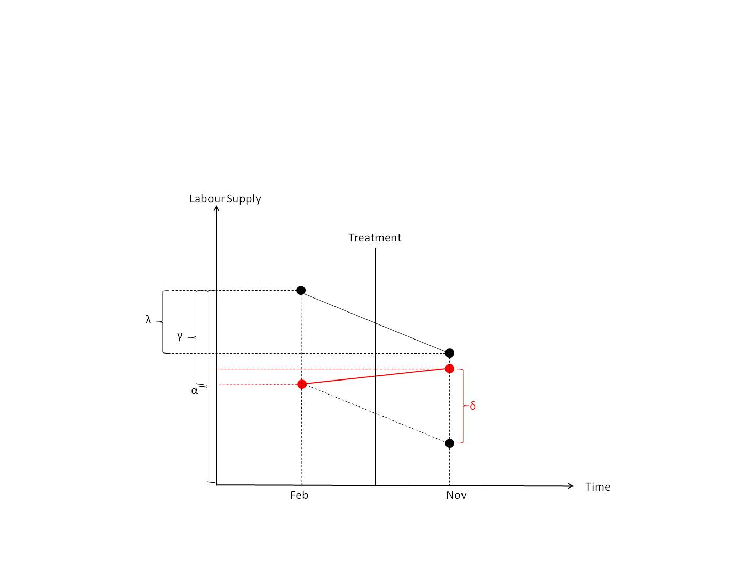
\includegraphics[scale=0.90]{./lecture_includes/waldinger_dd_5.pdf}
	\end{figure}
\end{frame}



	


\begin{frame}{Compositional differences violate parallel trends}
	
	\begin{itemize}
	\item One of the risks of a repeated cross-section is that the composition of the sample may have changed between the pre and post period
	\item Hong (2011) uses repeated cross-sectional data from the Consumer Expenditure Survey (CEX) containing music expenditure and internet use for a random sample of households
	\item Study exploits the emergence of Napter (first file sharing software widely used by Internet users) in June 1999 as a natural experiment
	\item Study compares internet users and internet non-users before and after emergence of Napster
	\end{itemize}

\end{frame}

\begin{frame}[plain]
	\begin{figure}
	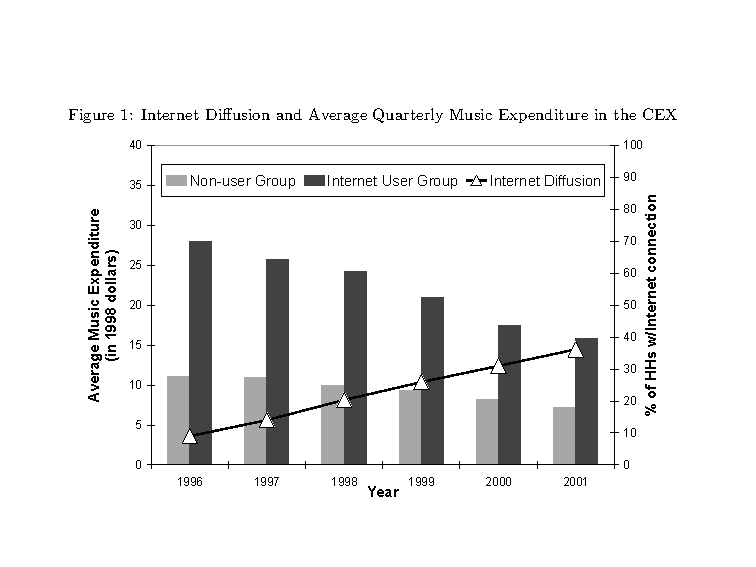
\includegraphics{./lecture_includes/Hong_1.pdf}
	\end{figure}
	
\end{frame}

\begin{frame}[shrink=20,plain]
	\begin{figure}
	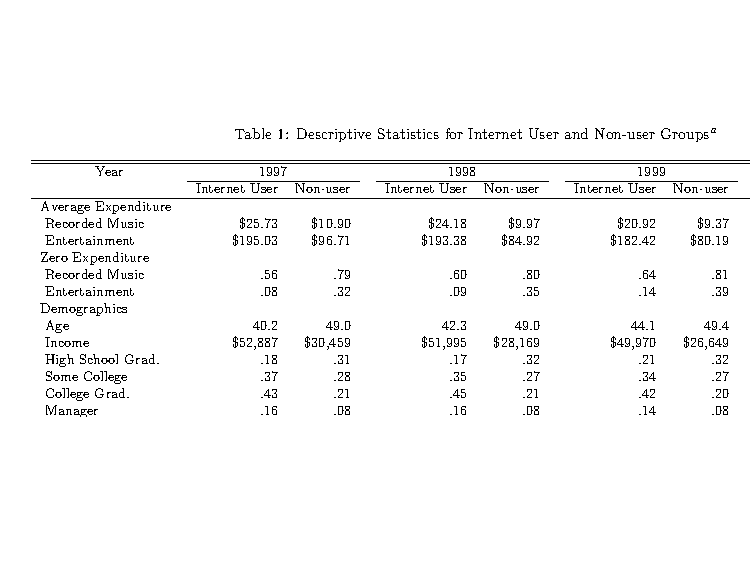
\includegraphics{./lecture_includes/Hong_2.pdf}
	\end{figure}
	
	Diffusion of the Internet changes samples (e.g., younger music fans are early adopters)
	
\end{frame}

\begin{frame}{Inference}
	
	\begin{itemize}
	\item  Bertrand, Duflo and Mullainathan (2004) show that conventional standard errors will often severely understate the standard deviation of the estimators
	\item Standard errors are biased downward (i.e., too small, over reject)
	\item They proposed three solutions, but most only use one of them (clustering)
	\end{itemize}
\end{frame}


\begin{frame}{Inference}
	
		\begin{enumerate}
		\item Block bootstrapping standard errors (if you analyze states the block should be the states and you would sample whole states with replacement for bootstrapping)
		\item Clustering standard errors at the group level (in Stata one would simply add \texttt{, cluster(state)} to the regression equation if one analyzes state level variation)
		\item Aggregating the data into one pre and one post period. Literally works if there is only one treatment data.  With staggered treatment dates one should adopt the following procedure:
			\begin{itemize}
			\item Regress $Y_{st}$ onto state FE, year FE and relevant covariates
			\item Obtain residuals from the treatment states only and divide them into 2 groups: pre and post treatment
			\item Then regress the two groups of residuals onto a post dummy
			\end{itemize}
		\end{enumerate}
\end{frame}


\subsection{Event study}

\begin{frame}{Evidence for parallel trends: pre-trends}

\begin{itemize}

	\item The identifying assumption for all DD designs is parallel trends, but since we cannot verify parallel trends, we often look at pre-trends
	\item But, even if pre-trends are the same one still has to worry about other policies changing at the same time (omitted variable bias)

\end{itemize}

\end{frame}

\begin{frame}{Plot the raw data when there's only two groups}

	\begin{figure}
	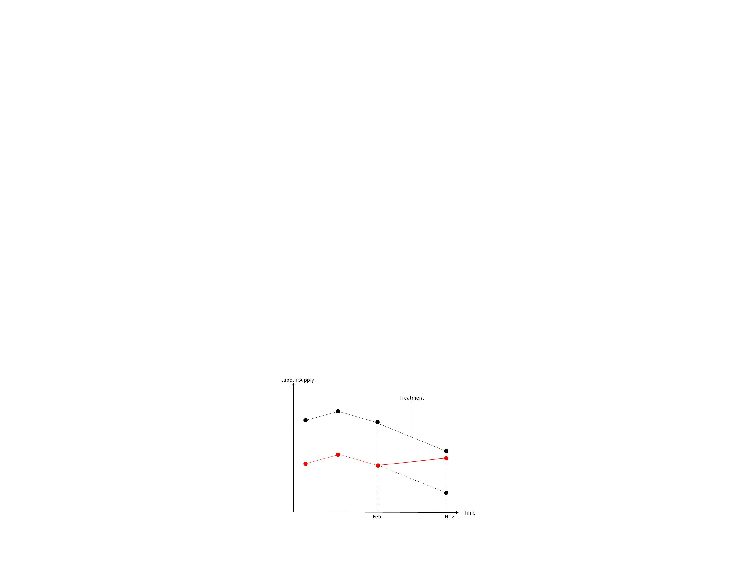
\includegraphics[scale=2.5]{./lecture_includes/waldinger_dd_6.pdf}
	\end{figure}

\end{frame}



\begin{frame}{Event study regression}
	
	\begin{itemize}
	\item Including leads into the DD model is an easy way to analyze pre-treatment trends
	\item Lags can be included to analyze whether the treatment effect changes over time after assignment
	\item The estimated regression would be:$$Y_{its} = \gamma_s + \lambda_t + \sum_{\tau=-2}^{-q}\mu_{\tau}D_{s\tau} + \sum_{\tau=0}^m\delta_{\tau}D_{s\tau}+\varepsilon_{ist}$$
		\begin{itemize}
		\item $D$ equals the treatment group interacted with the calendar year
		\item Treatment occurs in year 0, no anticipation, drop baseline $t-1$
		\item Includes $q$ leads or anticipatory effects
		\item Includes $m$ lags or post treatment effects
		\end{itemize}
	\end{itemize}
\end{frame}

\begin{frame}{Event study regression}


$$Y_{its} = \gamma_s + \lambda_t + \sum_{\tau=-2}^{-q}\mu_{\tau}D_{s\tau} + \sum_{\tau=0}^m\delta_{\tau}D_{s\tau}+\varepsilon_{ist}$$

\bigskip

Typically you'll plot the coefficients and 95\% CI on all leads and lags (binned or not, trimmed or not) 

\bigskip

Under parallel trends and no anticipation, then you expect $\widehat{\mu}$ coefficients to be zero, which gives you confidence that parallel trends holds (but is not a guarantee)

\end{frame}



\begin{frame}{Medicaid and Affordable Care Act example}

\begin{figure}
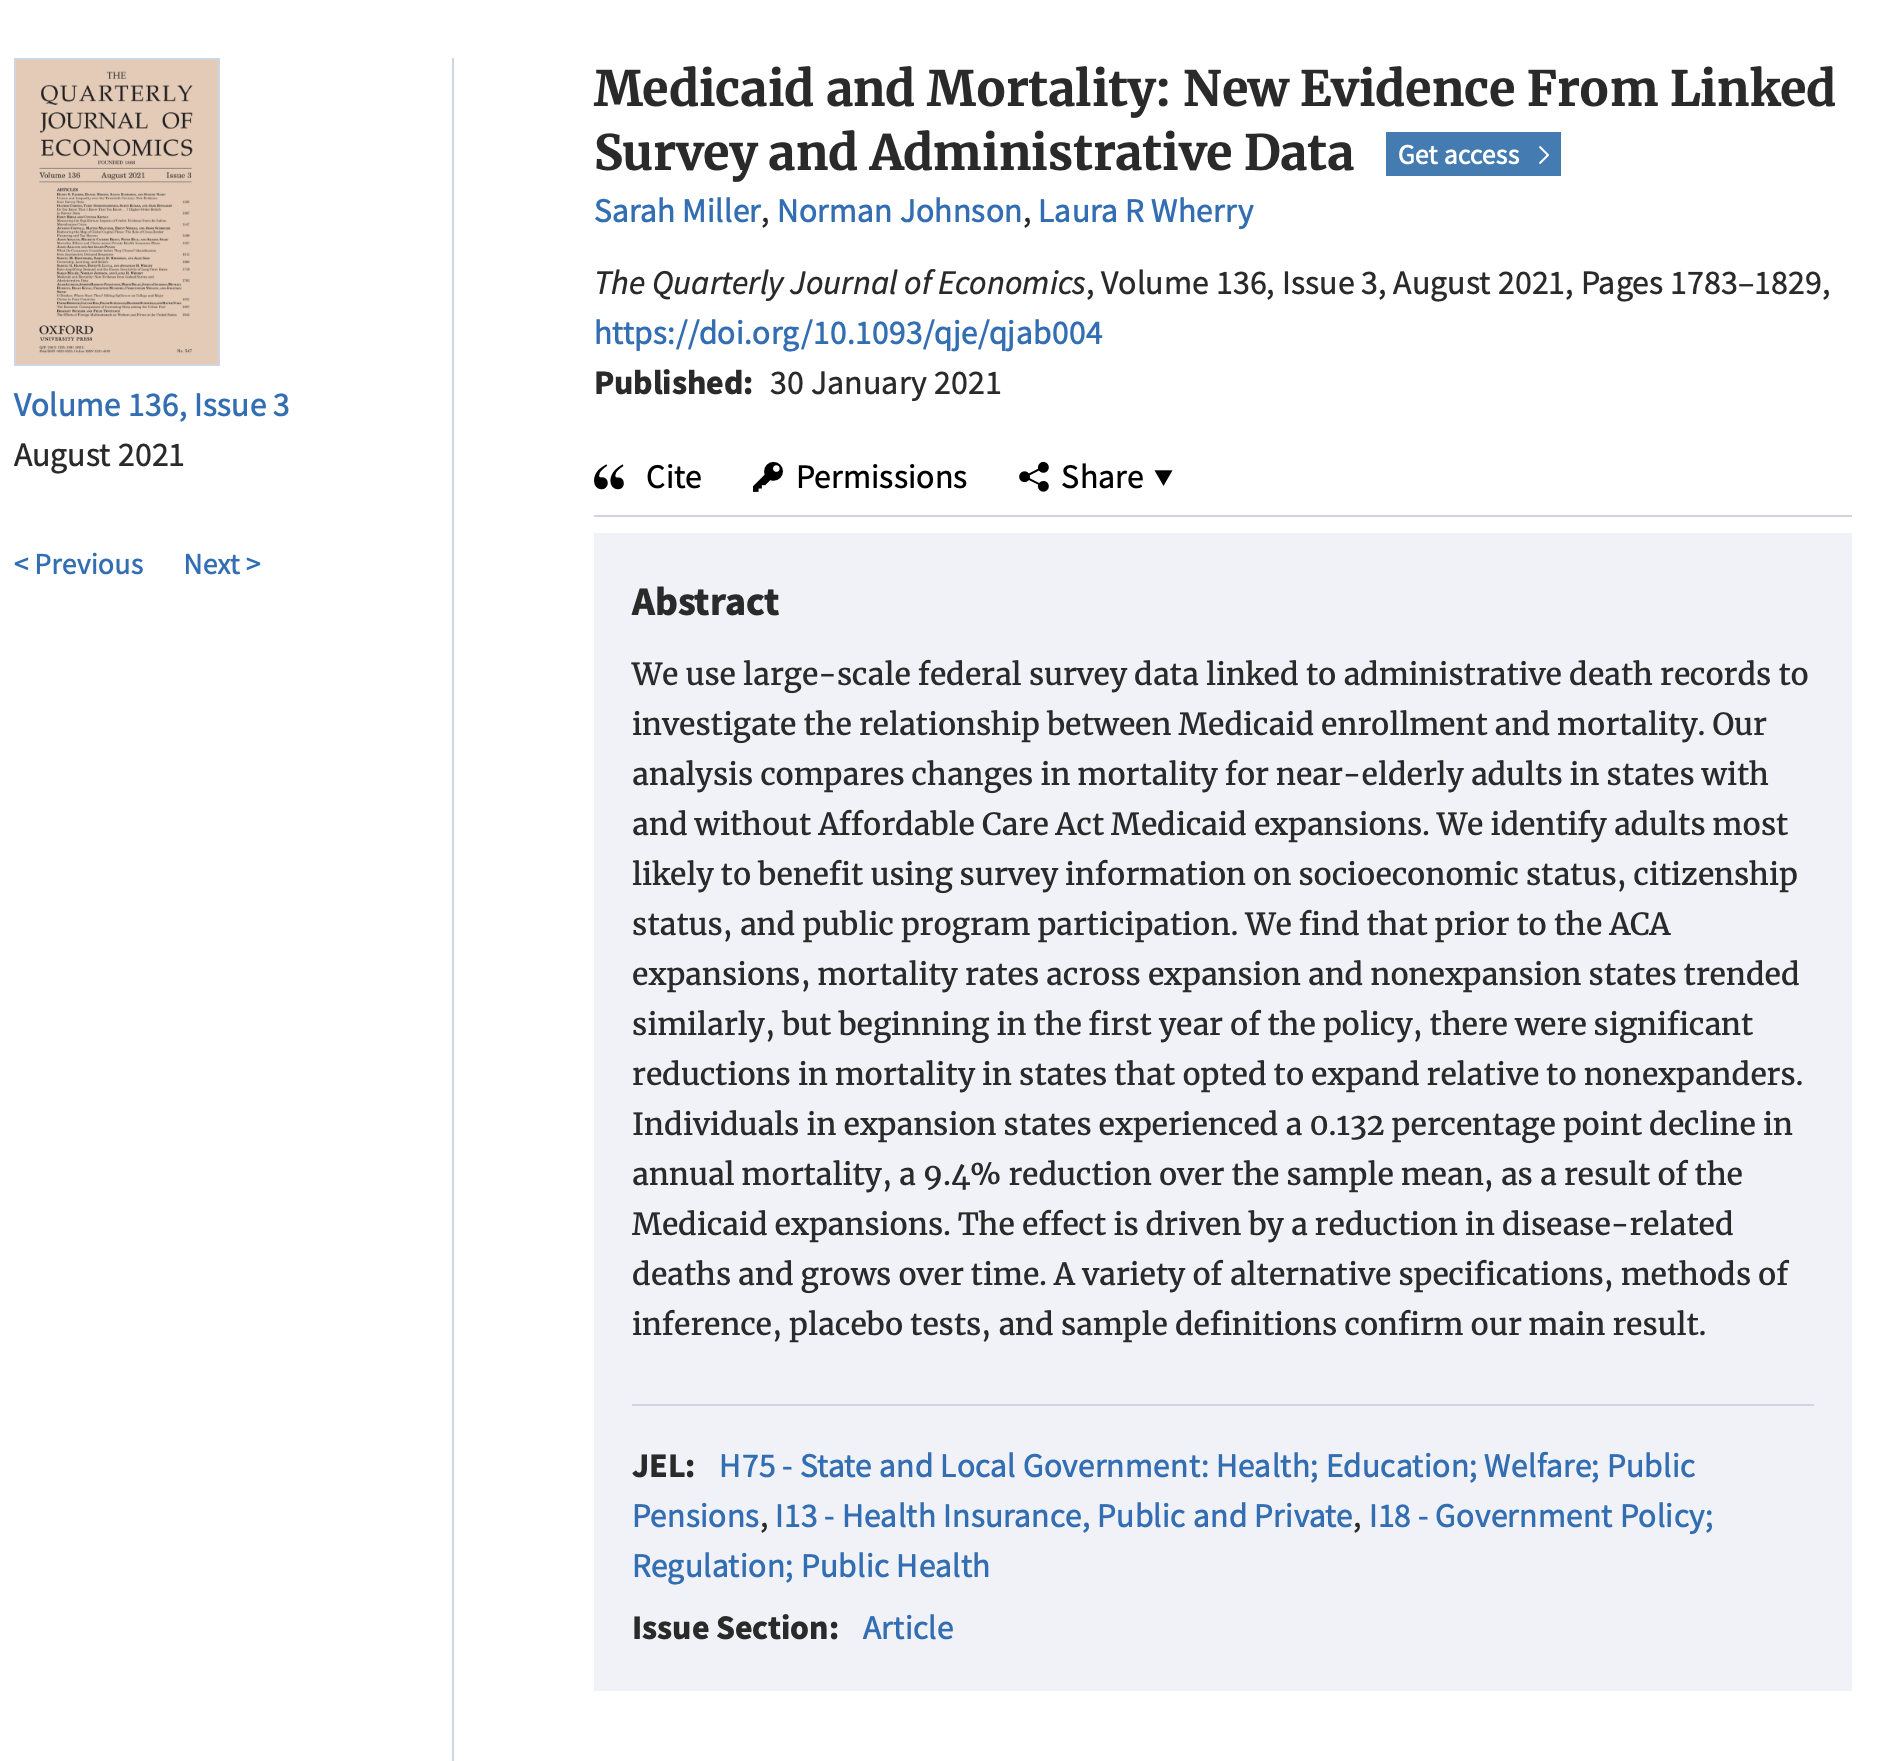
\includegraphics[scale=0.25]{./lecture_includes/medicaid_qje}
\end{figure}

\end{frame}

\begin{frame}{Evidence}

\begin{itemize}
\item \textbf{Bite} -- show that the expansion shifted people into Medicaid and out of uninsured status
\item \textbf{Placebos} -- Show that there's no effect on mortality for groups it shouldn't be affecting (people 65+)
\item \textbf{Event study} -- Show leads and lags on mortality
\end{itemize}

\end{frame}


\imageframe{./lecture_includes/Miller_Medicaid1.png}

\imageframe{./lecture_includes/Miller_Medicaid2.png}

\imageframe{./lecture_includes/Miller_Medicaid3.png}


\imageframe{./lecture_includes/medicaid_qje_placebo}


\begin{frame}[plain]

	\begin{figure}
	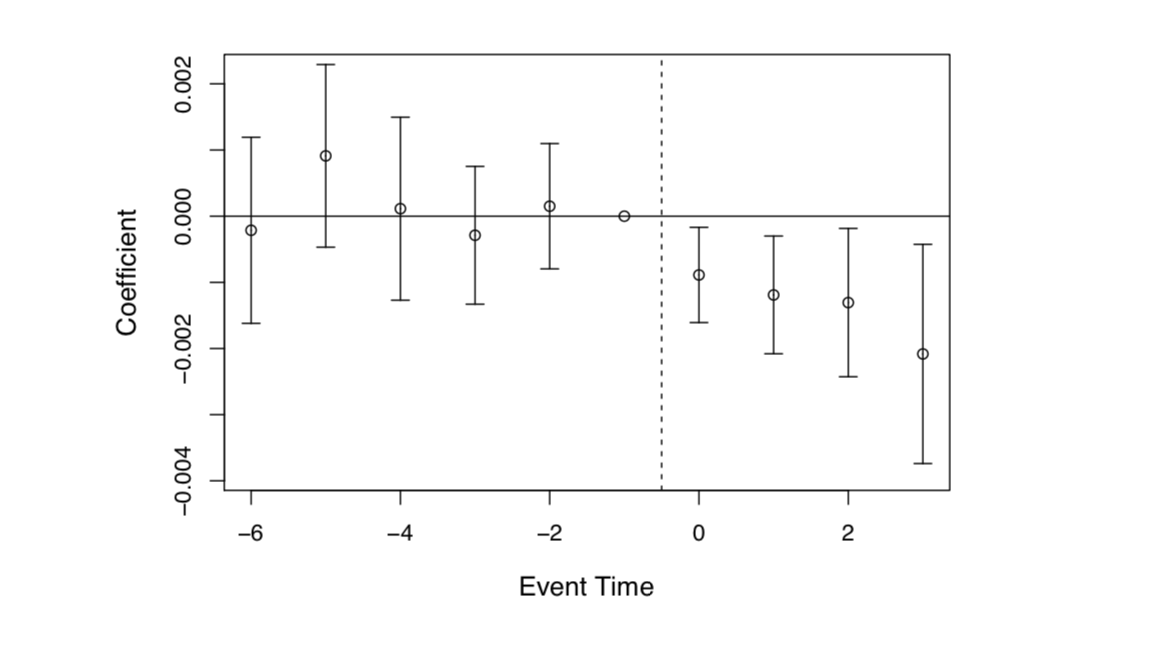
\includegraphics[scale=0.3]{./lecture_includes/Miller_Medicaid4.png}
	\caption{Miller, et al. (2019) estimates of Medicaid expansion's effects on on annual mortality}
	\end{figure}

\end{frame}

\subsection{Triple difference}

\begin{frame}{Additional identification things}
	
	\begin{itemize}
	\item Very common for readers and others to request a variety of ``robustness checks'' from a DD design
	\item Think of these as along the same lines as the event study we just discussed
		\begin{itemize}
		\item Falsification test using data for alternative control group (e.g., Medicare population)
		\item Falsification test using alternative ``placebo'' outcome that should not be affected by the treatment
		\end{itemize}
	\end{itemize}
\end{frame}


\begin{frame}[shrink=20]

\begin{table}\centering
		\caption{Difference-in-Difference-in-differences}
		\tiny
		\begin{center}
		\begin{tabular}{lll|l|lll}
		\hline \hline
		\multicolumn{1}{l}{\textbf{States}}&
		\multicolumn{1}{c}{\textbf{Group}}&
		\multicolumn{1}{c}{\textbf{Period}}&
		\multicolumn{1}{c}{\textbf{Outcomes}}&
		\multicolumn{1}{c}{$D_1$}&
		\multicolumn{1}{c}{$D_2$}&
		\multicolumn{1}{c}{$D_3$}\\
		\hline
		&&After	&$NJ+T+NJ_t+l_t+D$					\\
	&Low wage employment			&&&$T+NJ_t+l_t+D$			\\
		&&Before	&$NJ$					\\
NJ					&&&&&$D+l_t-s_t$			\\
		&&After	&$NJ+T+NJ_t+s_t$					\\
	&High wage employment		&&	&$T+NJ_t+s_t$				\\
		&&Before	&$NJ$					\\
								\\
&&&&&&$D$
\\
		&&After	&$PA+T+PA_t+l_t$				\\
	&Low wage employment			&&&$T+PA_t+l_t$ \\				
		&&Before	&$PA$					\\
PA					&&&&&$l_t-s_t$		\\
		&&After	&$PA+T+PA_t+s_t$					\\
	&High wage employment		&&&	$T+PA_t+s_t$				\\
		&&Before	&$PA$					\\
		\hline \hline
		\end{tabular}
		\end{center}
	\end{table}
	
\textbf{What is our identifying assumption?}

\bigskip

$l_t-s_t$ is the same for PA and NJ. That's the gap between high and low wage employment in PA (observed) is the same as NJ (counterfactual).



\end{frame}

\begin{frame}{DDD Example by Gruber}
	
	\begin{figure}
	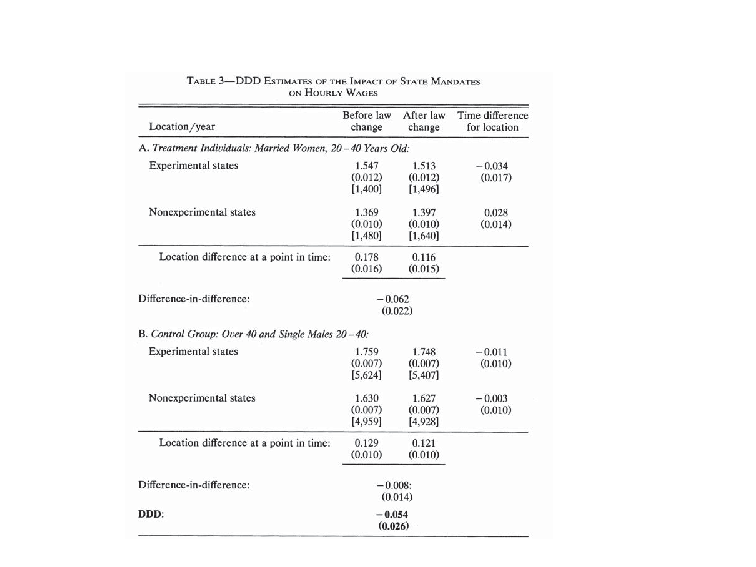
\includegraphics{./lecture_includes/gruber_ddd_3.pdf}
	\end{figure}
	
\end{frame}

\begin{frame}{DDD in Regression}
	
	\begin{eqnarray*}
	Y_{ijt} &=&\alpha +  \beta_2 \tau_t + \beta_3 \delta_j  + \beta_4 D_i + \beta_5(\delta \times \tau)_{jt} \\
	&& +\ \beta_6(\tau \times D)_{ti} +  \beta_7(\delta \times D)_{ij} +  \textcolor{red}{\beta_8(\delta \times \tau \times  D)_{ijt}}+  \varepsilon_{ijt}
	\end{eqnarray*}
	
	\begin{itemize}
	\item Your panel is now a group $j$ state $i$ (e.g., AR high wage worker 1991, AR high wage worker 1992, etc.)
	\item Assume we drop $\tau_t$ but I just want to show it to you for now.
	\item If the placebo DD is non-zero, it might be difficult to convince the reviewer that the DDD removed all the bias 
	\end{itemize}
	
\end{frame}


\subsection{Falsifications}

\begin{frame}{Falsification test with alternative outcome}
	
	\begin{itemize}
	\item The within-group control group (DDD) is a form of placebo analysis using the same \emph{outcome}
	\item But there are also placebos using a \emph{different} outcome -- but you need a hypothesis of mechanisms to figure out what is in fact a \emph{different outcome}
	\item Figure out what those are, and test them -- finding no effect raises the epistemological credibility of the first result, interestingly
	\item Cheng and Hoekstra (2013) examine the effect of castle doctrine gun laws on non-gun related offenses like grand theft auto and find no evidence of an effect
	\end{itemize}
\end{frame}



\begin{frame}{Rational addiction as a placebo critique}


Sometimes, an empirical literature may be criticized using nothing more than placebo analysis

\begin{quote}``A majority of [our] respondents believe the literature is a success story that demonstrates the power of economic reasoning.  At the same time, they also believe the empirical evidence is weak, and they disagree both on the type of evidence that would validate the theory and the policy implications. Taken together, this points to an interesting gap.  On the one hand, most of the respondents claim that the theory has valuable real world implications.  On the other hand, they do not believe the theory has received empirical support.''
\end{quote}

\end{frame}

\begin{frame}{Placebo as critique of empirical rational addiction}

\begin{itemize}
	\item Auld and Grootendorst (2004) estimated standard ``rational addiction'' models (Becker and Murphy 1988) on data with milk, eggs, oranges and apples.  
	\item They find these plausibly non-addictive goods are addictive, which casts doubt on the empirical rational addiction models.
\end{itemize}

\end{frame}

\begin{frame}{Placebo as critique of peer effects}

\begin{itemize}
	\item Several studies found evidence for ``peer effects'' involving inter-peer transmission of smoking, alcohol use and happiness tendencies
	\item Christakis and Fowler (2007) found significant network effects on outcomes like obesity
	\item Cohen-Cole and Fletcher (2008) use similar models and data and find similar network ``effects'' for things that \emph{aren't} contagious like acne, height and headaches
	\item Ockham's razor - given social interaction endogeneity (Manski 1993), homophily more likely explanation
\end{itemize}

\end{frame}



\section{Including Covariates}

\subsection{Inverse probability weighting}

\begin{frame}{Controls}

\begin{itemize}
\item Controls can address omitted variable bias (backdoor criterion), and they can improve precision
\item OLS can accommodate controls, and so we tend to include them so long as they are time varying 
\item But unfortunately, time varying covariates can create problems, especially if the treatment causes the covariates (bad controls, colliders)
\end{itemize}

\end{frame}






\begin{frame}{Inverse probability weighting DiD}

 Abadie (2005) incorporates baseline covariates into the propensity score which are then used as weights to estimate the ATT in a simple 3-step process
	\begin{enumerate}
	\item Calculate each unit's ``after minus before'' (DiD equation)
	\item Estimate the conditional probability of treatment based on baseline covariates (propensity score estimation)
	\item Weight the comparison group's DiD equation with the IPW
	\end{enumerate}

\end{frame}

\begin{frame}{Terms}

\begin{itemize}
\item $t$ is year of treatment which doesn't vary across units (so no differential timing)
\item $Y^1$ and $Y^0$ are potential outcomes (counterfactual versus actual)
\item $D$ is 1 or 0 based on group and time
\item $X_b$ are ``baseline'' covariates \textbf{only} -- they do not vary over time, which means propensity scores are estimated off the $b$ period \textbf{only}
\end{itemize}

\end{frame}

\begin{frame}{Assumptions}

Kind of common for this propensity score literature to only have two assumptions.  But usually the first conditional independence.  Now it is parallel trends because this is DD

\begin{enumerate}
\item Conditional parallel trends $$E[Y^0_t - Y^0_b|D=1,X_b] - E[Y^0_t - Y^0_t | D=0, X_b]$$ (Notice the $b$ subscript.  What is that you think?)
\item Common support $$Pr(D=1)>0; Pr(D=1|X)<1$$ Let's see a picture of common support that I drew.  Apologies it's horrible
\end{enumerate}

\end{frame}

\begin{frame}{Common support}

As we are identifying the ATT, we only need common support with respect to treated units

\bigskip

Your identify assumptions are always with respect to the missing covariates in other words and for the ATT, you are missing $Y^0$ for the treatment group

\bigskip

If we were estimating ATU, we'd be missing $Y^1$ for controls and need common support ($Y$ in treatment for all ranges of control), and for ATE we'd need both

\end{frame}

\begin{frame}{Visualizing propensity score to get common support}

	\begin{figure}
	\includegraphics[scale=0.05]{./lecture_includes/common_support_abadie.png}
	\end{figure}

\end{frame}

\begin{frame}{Definition and estimation}

Defining the ATT parameter of interest
\begin{equation}
ATT=E[Y^1_t - Y^0_t |D_t=1]
\end{equation}

\bigskip
Abadie's estimator
\begin{equation}
E\bigg [ \frac{Y_t - Y_b}{Pr(D_t=1)} \times \frac{D_t - Pr(D=1|X_b)}{1-Pr(D=1|X_b)} \bigg ]
\end{equation}


\end{frame}


\begin{frame}{Propensity scores}

\begin{itemize}
\item It's common to hear people say that we don't know the propensity score; we can only estimate it. Same here -- we approximate it with regressions
\item Paper is titled ``Semi-parametric DiD'' because Abadie imposes structure on the polynomials used to construct the propensity score (``series logit'')
\end{itemize}

\end{frame}



\begin{frame}{Abadie 2005 influence}

	\begin{figure}
	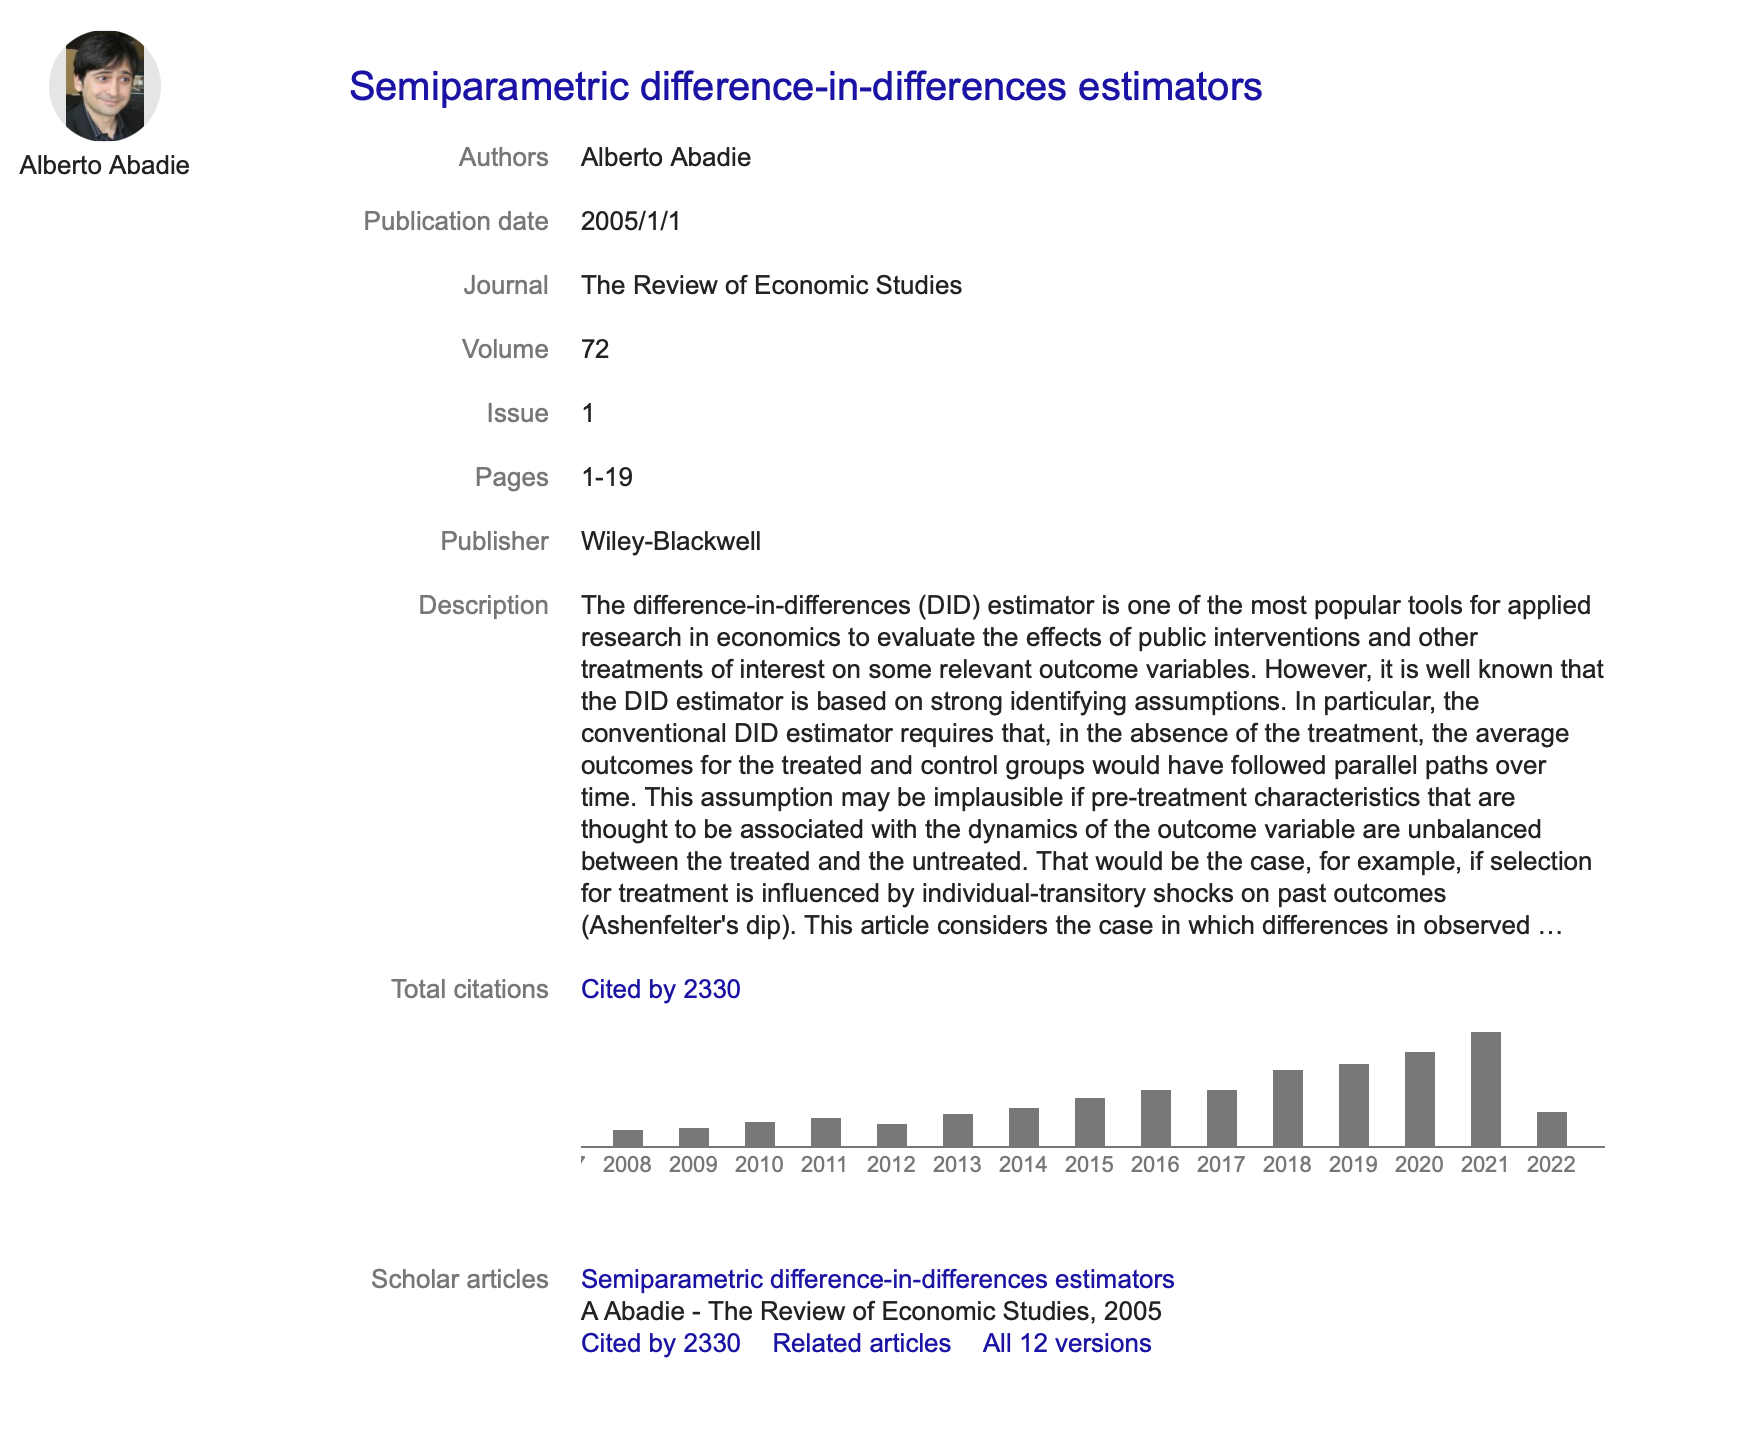
\includegraphics[scale=0.25]{./lecture_includes/abadie_restud_ipw}
	\end{figure}Abadie (2005) is his fourth most cited paper

\end{frame}




\subsection{Double Robust DiD}

\begin{frame}{Doubly Robust Difference-in-differences}

\begin{itemize}
\item DR models control for covariates twice -- once using the propensity score, once using outcomes adjusted by regression -- and are unbiased so long as:
	\begin{itemize}
	\item The regression specification for the outcome is correctly specified
	\item The propensity score specification is correctly specified
	\end{itemize}
\item Sant'Anna and Zhao (2020) incorporated DR into DiD by combining inverse probability weighting and outcome regression into a single DiD model
\item It's in the engine of Callaway and Sant'Anna (2020) that we discuss later so it merits close study
\item One of my favorite lesser known of the new DiD papers
\end{itemize}

\end{frame}

\begin{frame}{Patterns in econometrician reasoning}

\begin{enumerate}
\item Define the target parameter first (as opposed to writing down a regression specification first)
\item Identification (e.g., parallel trends)
\item Estimation
\item Aggregation
\item Inference
\end{enumerate}

\end{frame}


\begin{frame}{Defining the target parameter}

Major part of the new econometrics is to always start with the target parameter and build to it using estimation and identification that ``works''

\bigskip

\begin{eqnarray*}
\delta = E[Y^1_{it} - Y^0_{it} | D_i=1]
\end{eqnarray*}

\end{frame}

\begin{frame}{Identification assumptions I: Data}

Assumption 1: Assume panel data or repeated cross-sectional data

\bigskip

Handling repeated cross-sectional data is possible but assumes modularity which is a kind of stability assumption, but I'll use panel representation. 

\bigskip

Cross-sections will be potentially violated with changing sample compositions (e.g., the Napster example). 

\end{frame}

\begin{frame}{Identification assumptions II: Modification to parallel trends}

Assumption 2: Conditional parallel trends

\bigskip

Counterfactual trends for the treatment group are the same as the control group for all values of $X$

\begin{eqnarray*}
E[Y_1^0 - Y_0^0 | X, D=1] = E[Y^0_1 - Y^0_0 | X, D=0]
\end{eqnarray*}

\end{frame}

\begin{frame}{Identification assumptions III: Common support}

Assumption 3: Common support

\bigskip

For some $e>0$, the probability of being in the treatment group is greater than $e$ and the probability of being in the treatment group conditional on $X$ is $\leq1-e$. 

\bigskip

Intuition of assumption 3: Called overlap or common support. Means there is at least a small fraction of the population that is treated and that for every value of the covariates $X$ there is at least a small chance that the unit is not treated. It's called common support when it's a propensity score but it's just about the distribution of treatment and control across values of $X$. Very common when dealing with covariate comparisons as otherwise you're extrapolating (curse of dimensionality)

\end{frame}

\begin{frame}{Estimating DD with Assumptions 1-3}

\begin{itemize}
\item Assumptions 1-3 gives us a couple of options of estimating the DiD
\item We can either use the outcome regression (OR) approach of Heckman, et al 1997
\item Or we can use the inverse probability weighting (IPW) approach of Abadie (2005)
\end{itemize}

\end{frame}


\begin{frame}{Heckman, et al. 1997}

	\begin{figure}
	
\includegraphics[scale=0.35]{./lecture_includes/petra_restud_1997}
	\end{figure}

\end{frame}



\begin{frame}{Outcome regression}

This is the Heckman, et al. (1997) approach where the outcome evolution is modeled with a regression

\bigskip

\begin{eqnarray*}
\widehat{\delta}^{OR} = \overline{Y}_{1,1} - \bigg [ \overline{Y}_{1,0} + \frac{1}{n^T} \sum_{i|D_i=1} ( \widehat{\mu}_{0,1}(X_i) - \widehat{\mu}_{0,0}(X_i)) \bigg ]
\end{eqnarray*}

where $\overline{Y}$ is the sample average of $Y$ among units in the treatment group at time $t$ and $\widehat{\mu}(X)$ is an estimator of the true, but unknown, $m_{d,t}(X)$ which is by definition equal to $E[Y_t|D=d,X=x]$.

\end{frame}




\begin{frame}{Outcome regression}

\begin{eqnarray*}
\widehat{\delta}^{OR} = \overline{Y}_{1,1} - \bigg [ \overline{Y}_{1,0} + \frac{1}{n^T} \sum_{i|D_i=1} ( \widehat{\mu}_{0,1}(X_i) - \widehat{\mu}_{0,0}(X_i)) \bigg ]
\end{eqnarray*}

\begin{enumerate}
\item Regress changes $\Delta Y$ on $X$ among untreated groups using baseline covariates only
\item Get fitted values of the regression using all $X$ from $D=1$ only.  Average those
\item Calculate change in this fitted $Y$ among treated with the average fitted values
\end{enumerate}

\end{frame}

\begin{frame}{Inverse probability weighting}

This is the Abadie (2005) approach where we use weighting

\begin{eqnarray*}
\widehat{\delta}^{ipw} = \frac{1}{E_N[D]} E \bigg [ \frac{D-\widehat{p}(X)}{1-\widehat{p}(X)} (Y_1-Y_0) \bigg ]
\end{eqnarray*}

where $\widehat{p}(X)$ is an estimator for the true propensity score. Reduces the dimensionality of $X$ into a single scalar.

\end{frame}

\begin{frame}{These models cannot be ranked}

\begin{itemize}
\item Outcome regression needs $\widehat{\mu}(X)$ to be correctly specified, whereas
\item Inverse probability weighting needs $\widehat{p}(X)$ to be correctly specified
\item It's hard to ``rank'' these two in practice with regards to model misspecification because each is inconsistent when their own models are misspecified
\end{itemize}

\end{frame}


\begin{frame}{TWFE}

Consider our earlier TWFE specification:

\begin{eqnarray*}
Y_{it} = \alpha_1  + \alpha_2 T_t + \alpha_3 D_i +  \delta (T_i \times D_t)  + \varepsilon_{it}
\end{eqnarray*}

\bigskip

Just add in covariates then right?

\begin{eqnarray*}
Y_{it} = \alpha_1  + \alpha_2 T_t + \alpha_3 D_i  + \delta (T_i \times D_t) + \theta \cdot X_{it} + \varepsilon_{it}
\end{eqnarray*}

Sure! If you're willing to impose three \emph{more} assumptions

\end{frame}




\begin{frame}{Decomposing TWFE with covariates}

TWFE places restrictions on the DGP. Previous TWFE regression under assumptions 1-3 implies the following:

\bigskip

\begin{eqnarray*}
E[Y^1_1|D=1,X] = \alpha_1 + \alpha_2 + \alpha_3 + \delta + \theta X
\end{eqnarray*}

\bigskip

Conditional parallel trends implies

\small
\begin{eqnarray*}
&&E[Y^0_{1} - Y^0_{0}|D=1,X]= E[Y^0_{1} - Y^0_{0}|D=0,X] \\
&&E[Y^0_{1}|D=1,X] - E[Y^0_{0}|D=1,X]= E[Y^0_{1}|D=0,X] - E[Y^0_{0}|D=0,X] \\
&&E[Y^0_{1}|D=1,X] = E[Y^0_{0}|D=1,X] + E[Y^0_{1}|D=0,X] - E[Y^0_{0}|D=0,X] \\
&&E[Y^0_{1}|D=1,X] = E[Y_{0}|D=1,X] + E[Y_{1}|D=0,X] - E[Y_{0}|D=0,X] \\
\end{eqnarray*}


\end{frame}

\begin{frame}{Switching equation substitution}

Last line from the switching equation. This gives us:

\begin{eqnarray*}
E[Y^0_{1}|D=1,X] = \alpha_1  + \alpha_2 + \alpha_3 + \theta X
\end{eqnarray*}

Now compare this with our earlier $Y^1$ expression

\begin{eqnarray*}
E[Y^1_1|D=1,X] = \alpha_1 + \alpha_2 + \alpha_3 + \delta + \theta X
\end{eqnarray*}

We can define our target parameter, the ATT, now in terms of the fixed effects representation

\end{frame}


\begin{frame}{Collecting terms}

TWFE representation of our conditional expectations of the potential outcomes
\begin{eqnarray*}
&&E[Y^1_1|D=1,X] = \alpha_1 + \alpha_2 + \alpha_3 + \delta + \theta_1 X \\
&&E[Y^0_{1}|D=1,X] = \alpha_1  + \alpha_2 + \alpha_3 + \theta_2 X \\
\end{eqnarray*}

Substitute these into our target parameter

\begin{eqnarray*}
ATT &=& E[Y^1_1|D=1,X]  - E[Y^0_{1}|D=1,X]   \\
&&=(\alpha_1 + \alpha_2 + \alpha_3 + \delta + \theta_1 X) - ( \alpha_1  + \alpha_2 + \alpha_3 + \theta_2 X )\\
&&=\delta + (\theta_1 X - \theta_2 X)
\end{eqnarray*}

\bigskip

What if $\theta_1 X \neq \theta_2 X$?

\end{frame}

\begin{frame}{Assumption 4: Homogeneous treatment effects in X}


TWFE requires homogenous treatment effects in $X$ (i.e., the treatment effect is the same for all $X$)

\bigskip

If $X$ is sex, then effects are the same for males and females.

\bigskip

  If $X$ is continuous, like income, then the effect is the same whether someone makes \$1 or \$1 million.

\end{frame}

\begin{frame}{X-specific trends}

TWFE also places restrictions on covariate trends for the two groups too.  Take conditional expectations of our TWFE equation. 

\begin{eqnarray*}
E[Y_1|D=1] &=& \alpha_1 + \alpha_2 + \alpha_3 + \delta + \theta X_{11} \\
E[Y_0|D=1] &=& \alpha_1 + \alpha_3 + \theta X_{10} \\
E[Y_1|D=0] &=& \alpha_1 + \alpha_2 + \theta X_{01} \\
E[Y_0|D=0] &=& \alpha_1 + \theta X_{00}
\end{eqnarray*}


\end{frame}


\begin{frame}{X-specific trends}

Now take the DiD formula:

\begin{eqnarray*}
\delta^{DD} = &&\bigg ( (\alpha_1 + \alpha_2 + \alpha_3 + \delta + \theta X_{11} ) - (\alpha_1 + \alpha_3 + \theta X_{10} ) \bigg )- \\
&& \bigg ( (\alpha_1 + \alpha_2 + \theta X_{01}) - (\alpha_1 + \theta X_{00}) \bigg )
\end{eqnarray*}

\bigskip

Eliminating terms, we get:

\begin{eqnarray*}
\delta^{DD} = &&\delta + \\
&& (\theta X_{11} - \theta X_{10} ) - (\theta X_{01} - \theta X_{00} )
\end{eqnarray*}

\bigskip

Second line requires that trends in X for treatment group equal trends in X for control group.

\end{frame}


\begin{frame}{Assumption 5 and 6}

We need ``no X-specific trends'' for the treatment group (assumption 5) and comparison group (assumption 6)

\bigskip

\textbf{Intuition}: No X-specific trends means the evolution of potential outcome $Y^0$ is the same regardless of $X$. This would mean you cannot allow rich people to be on a different trend than poor people, for instance.

\bigskip

Without these six, in general TWFE will not identify ATT. 

\end{frame}

\begin{frame}{Why not both?}

\begin{itemize}
\item Let's review the problem.  What if you claim you need $X$ for conditional parallel trends?
\item You have three options:
	\begin{enumerate}
	\item Outcome regression (Heckman, et al. 1997) -- needs Assumptions 1-3
	\item Inverse probability weighting (Abadie 2005) -- needs Assumptions 1-3
	\item TWFE (everybody everywhere all the time) -- needs Assumptions 1-6
	\end{enumerate}
\item Problem is 1 and 2 need the models to be correctly specified
\item Doubly robust combines them to give us insurance; we now get two chances to be wrong, as opposed to just one
\end{itemize}

\end{frame}


\begin{frame}{Double Robust DiD}
\begin{eqnarray*}
\delta^{dr} = E \bigg [ \bigg ( \frac{D}{E[D]} -\frac{ \frac{p(X)(1-D)}{(1-p(X))} }{E \bigg [\frac{p(X)(1-D)}{(1-p(X))} \bigg ]} \bigg  )( \Delta Y - \mu_{0,\Delta}(X)) \bigg ]
\end{eqnarray*}

\begin{eqnarray*}
&&p(x): \text{propensity score model} \\
&& \Delta Y = Y_1 - Y_0 = Y_{post} - Y_{pre} \\
&& \mu_{d,\Delta} = \mu_{d,1}(X) - \mu_{d,0}(X), \text{ where } \mu(X) \text{ is a model for} \\
&& m_{d,t} = E[Y_t|D=d,X=x]
\end{eqnarray*}So that means $\mu_{0,\Delta}$ is just the control group's change in average $Y$ for each $X=x$

\end{frame}

\begin{frame}{Double Robust DiD}

\begin{eqnarray*}
\delta^{dr} = E \bigg [ \bigg ( \frac{D}{E[D]} -\frac{ \frac{p(X)(1-D)}{(1-p(X))} }{E \bigg [\frac{p(X)(1-D)}{(1-p(X))} \bigg ]} \bigg  )( \Delta Y - \mu_{0,\Delta}(X)) \bigg ]
\end{eqnarray*}

Notice how the model controls for $X$: you're weighting the adjusted outcomes using the propensity score

\bigskip

The reason you control for $X$ twice is because you don't know which model is right.  DR DiD frees you from making a choice without making you pay too much for it


\end{frame}

\begin{frame}{Efficiency}

\begin{itemize}
\item Authors exploit all the restrictions implied by the assumptions to construct semiparametric bounds
\item This is where the influence function comes in, which those who have studied the DID code closely may have noticed
\item One of the main results of the paper is that the DR DiD estimator is also DR for inference
\item Let's skip to Monte Carlos
\end{itemize}

\end{frame}

\begin{frame}{Monte Carlo details}

\begin{itemize}
\item Compare DR with TWFE, OR and IPW
\item Sample size is 1,000
\item 10,000 Monte Carlo experiments
\item Propensity score estimated with logit; OR estimated using linear specification
\end{itemize}

\end{frame}



\begin{frame}[plain]

\begin{table}[htbp]\centering
\scriptsize
\caption{Monte Carlo Simulations, DGP1, Both OR and Propensity score correct}
\centering
\begin{threeparttable}
\begin{tabular}{l*{5}{c}}
\toprule
\multicolumn{1}{l}{\textbf{}}&
\multicolumn{1}{c}{\textbf{Bias}}&
\multicolumn{1}{c}{\textbf{RMSE}}&
\multicolumn{1}{c}{\textbf{SE}}&
\multicolumn{1}{c}{\textbf{Coverage}}&
\multicolumn{1}{c}{\textbf{CI length}}\\
\midrule
TWFE & -20.9518 & 21.1227 & 2.5271 & 0.000 & 9.9061 \\
OR & -0.0012 & 0.1005 & 0.1010 & 0.9500 & 0.3960 \\
IPW & 0.0257 & 2.7743 & 2.6636 & 0.9518 & 10.4412 \\
DR & -0.0014 & 0.1059 & 0.1052 & 0.9473 & 0.4124 \\
\bottomrule
\end{tabular}
\end{threeparttable}
\end{table}

\end{frame}


\begin{frame}[plain]
	\begin{figure}
	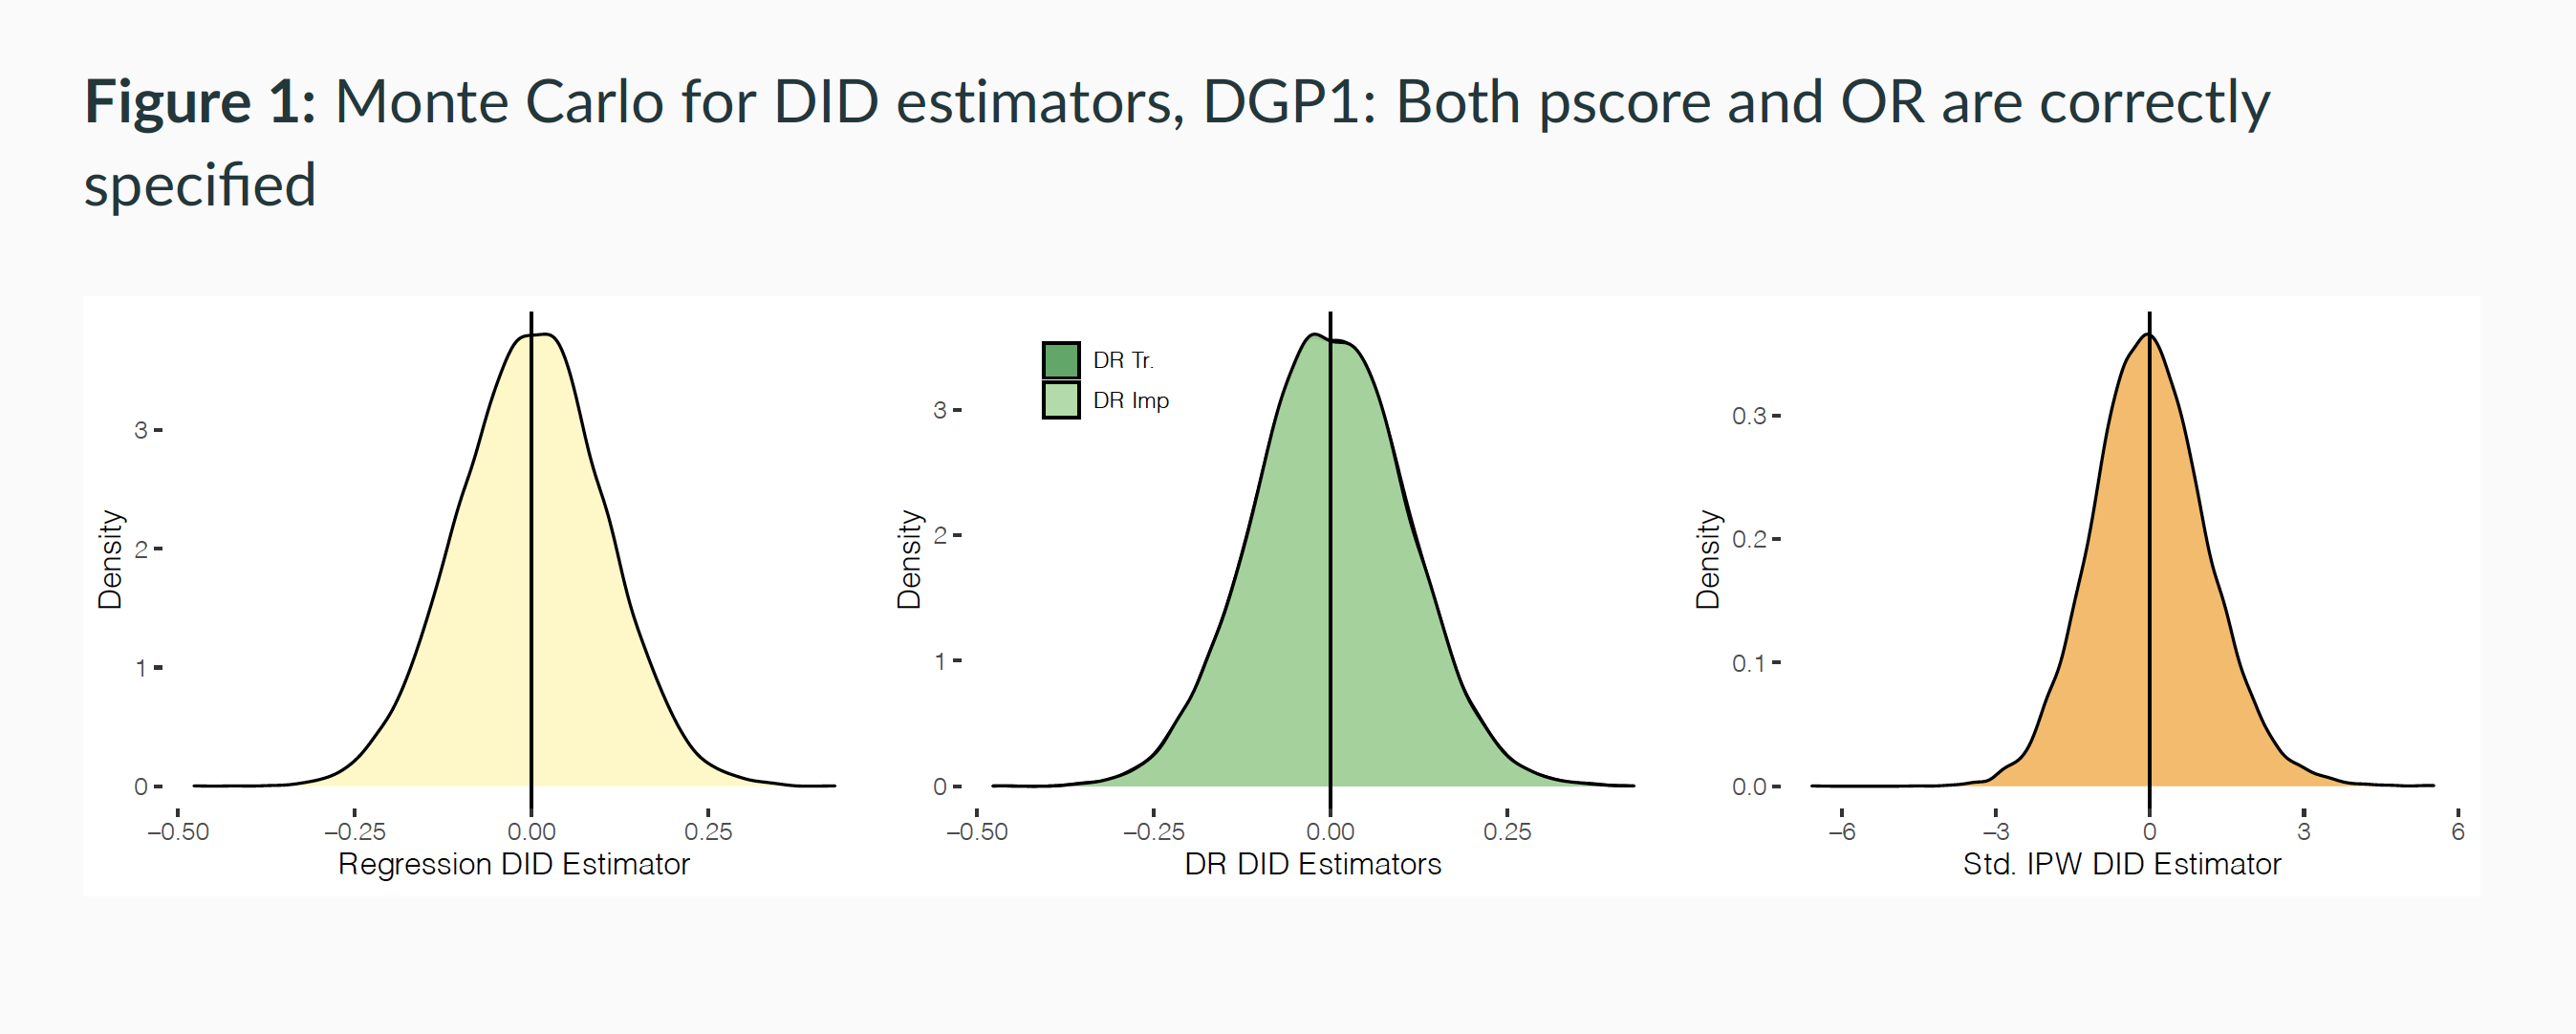
\includegraphics[scale=0.25]{./lecture_includes/mc_dr_1.png}
	\end{figure}

\end{frame}


\begin{frame}[plain]

\begin{table}[htbp]\centering
\scriptsize
\caption{Monte Carlo Simulations, DGP4, Neither OR and Propensity score correct}
\centering
\begin{threeparttable}
\begin{tabular}{l*{5}{c}}
\toprule
\multicolumn{1}{l}{\textbf{}}&
\multicolumn{1}{c}{\textbf{Bias}}&
\multicolumn{1}{c}{\textbf{RMSE}}&
\multicolumn{1}{c}{\textbf{SE}}&
\multicolumn{1}{c}{\textbf{Coverage}}&
\multicolumn{1}{c}{\textbf{CI length}}\\
\midrule
TWFE & -16.3846 & 16.5383 & 3.6268 & 0.000 & 14.2169 \\
OR & -5.2045 & 5.3641 & 1.2890 & 0.0145 & 5.0531 \\
IPW & -1.0846 & 2.6557 & 2.3746 & 0.9487 & 9.3084 \\
DR & -3.1878 & 3.4544 & 1.2946 & 0.3076 & 5.0749 \\
\bottomrule
\end{tabular}
\end{threeparttable}
\end{table}

\end{frame}

\begin{frame}[plain]
	\begin{figure}
	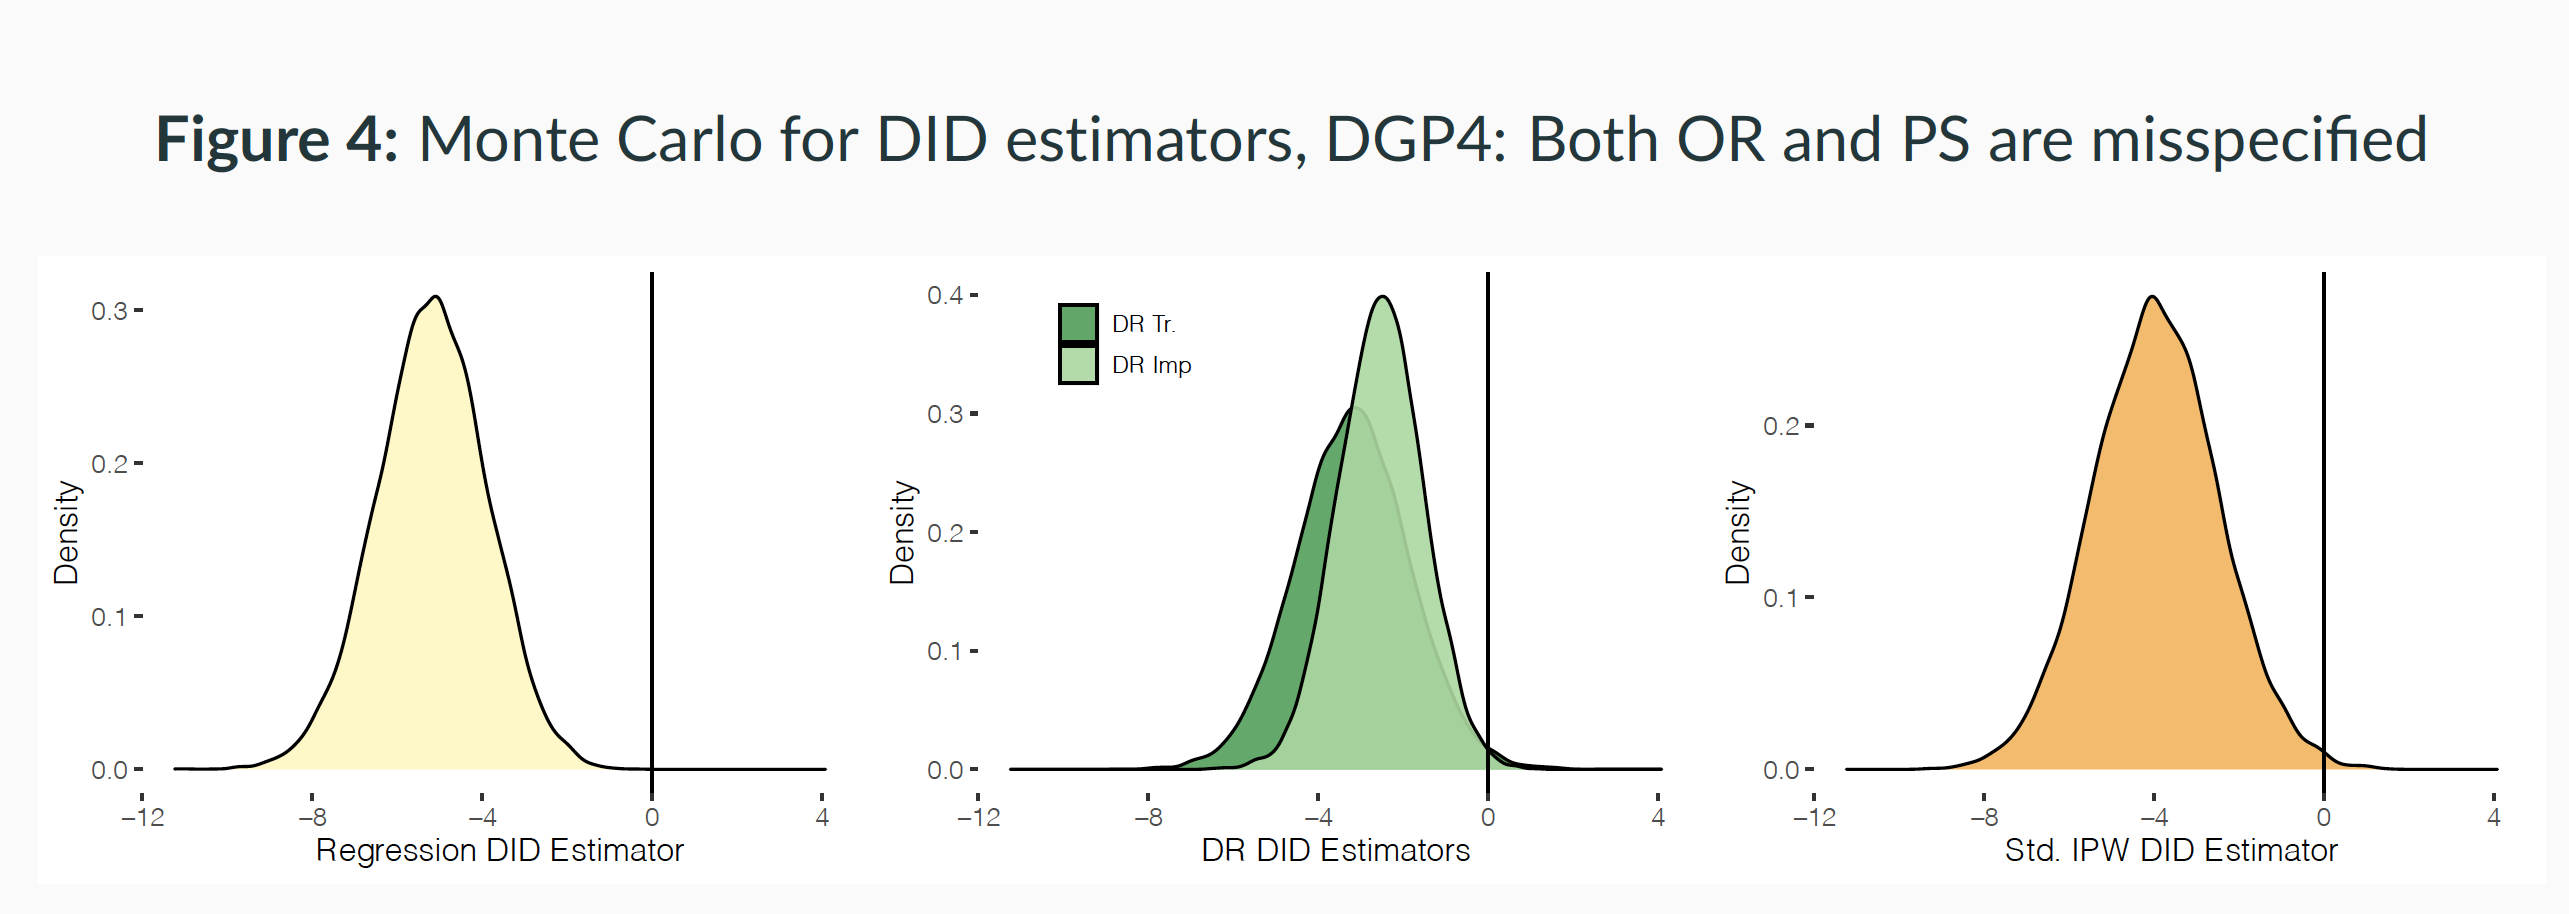
\includegraphics[scale=0.12]{./lecture_includes/mc_dr_2.png}
	\end{figure}


\end{frame}


\begin{frame}{Code}

There is code in R and Stata
\begin{itemize}
\item Stata: \textbf{drdid}
\item R: \textbf{drdid}
\end{itemize}
\bigskip
Remember -- it's for 2x2 with covariates (i.e., one treatment group)

\end{frame}




\begin{frame}{Concluding remarks}

\begin{itemize}
\item So we hopefully see a few of the key elements of DiD
	\begin{itemize}
	\item DiD equation and ATT equation are distinct
	\item Pre-trends is a placebo for evaluating parallel trends
	\item DiD is a design; OLS is a model
	\end{itemize}
\item Including covariates posed problems for the canonical OLS specification
\item Problem with that OLS specification was \emph{the specification}, not OLS -- it assumed constant treatment effects
\end{itemize}

\end{frame}


\end{document}
